\documentclass[conf]{new-aiaa}
%\documentclass[journal]{new-aiaa} for journal papers
\usepackage[utf8]{inputenc}

\usepackage{graphicx}
\usepackage{amsmath}
\usepackage[version=4]{mhchem}
\usepackage{siunitx}
\usepackage{longtable,tabularx}
\setlength\LTleft{0pt} 

\title{AE 5335 Final Exam}
\author{Riley J. Kyle} 

\begin{document}

\maketitle



\clearpage

\begin{figure}[hbt!]
    \centering
    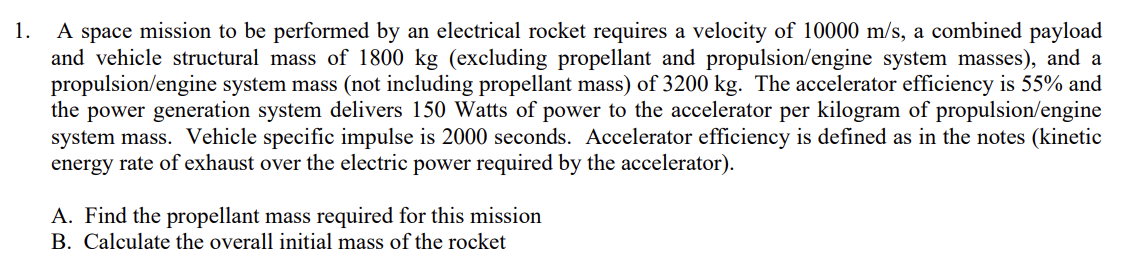
\includegraphics[width=1\textwidth]{images/1.png}
\end{figure}

\noindent The propellant mass is:

\begin{equation*}
    m_p = m_d \left(e^{\frac{\delta v}{C}}-1\right) = \boxed{3323.825\;kg}
\end{equation*}

\noindent The overall initial mass is:

\begin{equation*}
    m_0 = m_e + m_L + m_p = m_d + m_p = \boxed{8323.825\;kg}
\end{equation*}


\clearpage
\begin{figure}[hbt!]
    \centering
    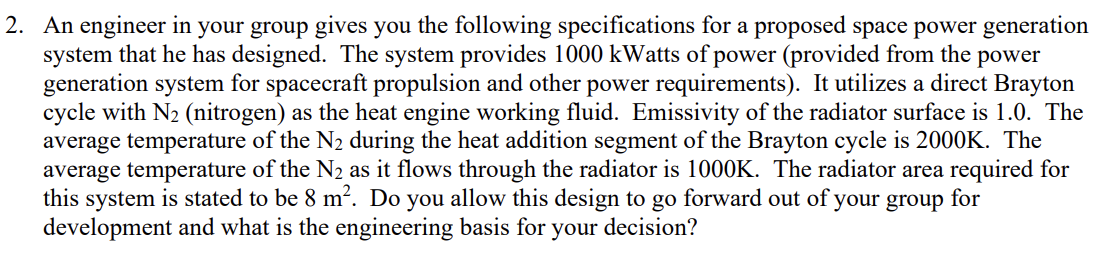
\includegraphics[width=1\textwidth]{images/2.png}
\end{figure}

\noindent For this problem I calculate the Carnot and Brayton efficiency.\\

\noindent The following is the Carnot efficiency:

\begin{equation*}
    \eta_c = 1 - \frac{T_L}{T_H} = 1 - \frac{T_{rad}}{T_{heat}} = 50\%
\end{equation*}

\noindent The following equation applies for any cycle:

\begin{equation*}
    \frac{A_{rad}}{W_{out}} = \frac{1}{\epsilon \sigma T_{R}^4} \left(\frac{1}{\eta} - 1\right)
\end{equation*}

\noindent Solving for the efficiency gives:

\begin{equation*}
    \eta_b = 69\%
\end{equation*}

This design should \textbf{not} move forward. The Carnot efficiency is less than that of the Brayton efficiency.
This shows that there is a violation of the second law of thermodynamics.




\clearpage
\begin{figure}[hbt!]
    \centering
    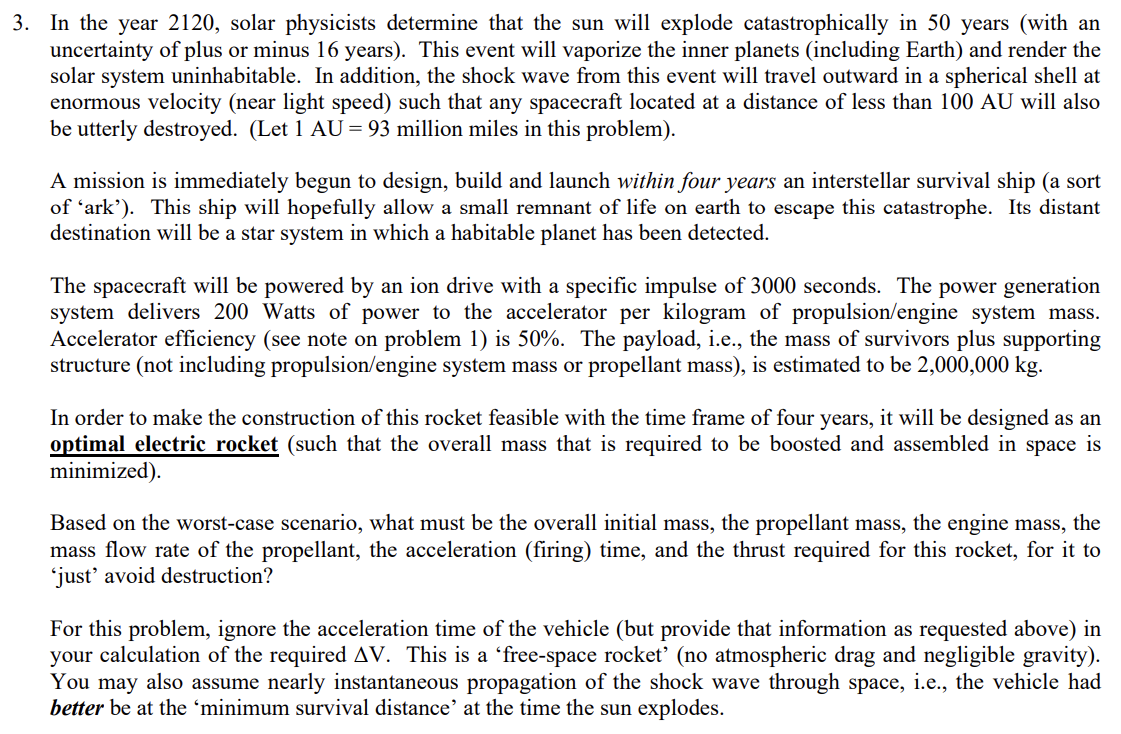
\includegraphics[width=1\textwidth]{images/3.png}
\end{figure}

\noindent The time left for the worst case is:

\begin{equation*}
    time = 50 - 16 - 4 = 30\;years = 946,080,000\;sec 
\end{equation*}

\noindent The distance traveled in meters is:

\begin{equation*}
    distance = 1.49669\times 10^{13}\;m
\end{equation*}

\noindent By ignoring the acceleration time the following is true:

\begin{equation*}
    V_{cruise} = \Delta V = \frac{distance}{time} = 15819.9\;m/s
\end{equation*}

\noindent Effective velocity:

\begin{equation*}
    C = I_{sp} g_0 = 28430\;m/s  
\end{equation*}

\noindent For convenience:
\begin{equation*}
    \alpha = \frac{\Delta V}{C}  
    = 0.5375
\end{equation*}
\begin{equation*}
    \beta = \beta_{opt} = \alpha  \left(\frac{\alpha}{\left(2\left(e^{\alpha} - 1\right) - \alpha\right)}\right)^{1/2}
    = 0.4187
\end{equation*}



\noindent Find the burn time:

\begin{equation*}
    \tau_b =  \left(\frac{\Delta V}{\beta}\right)^2\frac{1}{2\alpha^{\prime}\eta_a} = \boxed{82.619\;days}
\end{equation*}


\noindent The initial mass is:
\begin{equation*}
    m_0 = \frac{m_L}{\left(1 - \left(1 - e^{-\alpha}\right)\right)\left[1+\frac{\beta}{\alpha}^2\right]}
    =  \boxed{6,025,636\;kg}
\end{equation*}

\noindent The propellant mass is:
\begin{equation*}
    m_p = m_0 \left(1 - e^{\frac{\Delta V}{C}}\right)
    =  \boxed{2,505,571\;kg}
\end{equation*}

\noindent The propellant mass flow rate is:

\begin{equation*}
    \dot{m_p} = \frac{m_p}{\tau_b}
    =  \boxed{0.351\;kg/s}
\end{equation*}

\noindent The optimal engine mass is:

\begin{equation*}
    \dot{m_e} = m_0 - \left(m_L - m_p\right)
    =  \boxed{1,520,065\;kg}
\end{equation*}

\noindent The thrust required is:

\begin{equation*}
    Thrust = \dot{m_p} C
    =  \boxed{10,330\;N}
\end{equation*}


\clearpage
\begin{figure}[hbt!]
    \centering
    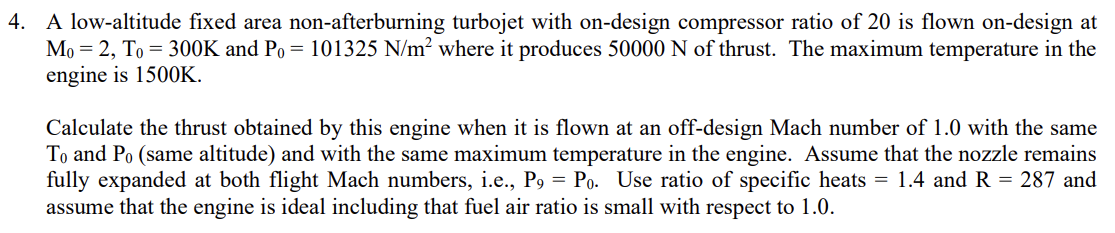
\includegraphics[width=1\textwidth]{images/4.png}
\end{figure}




\clearpage
\begin{figure}[hbt!]
    \centering
    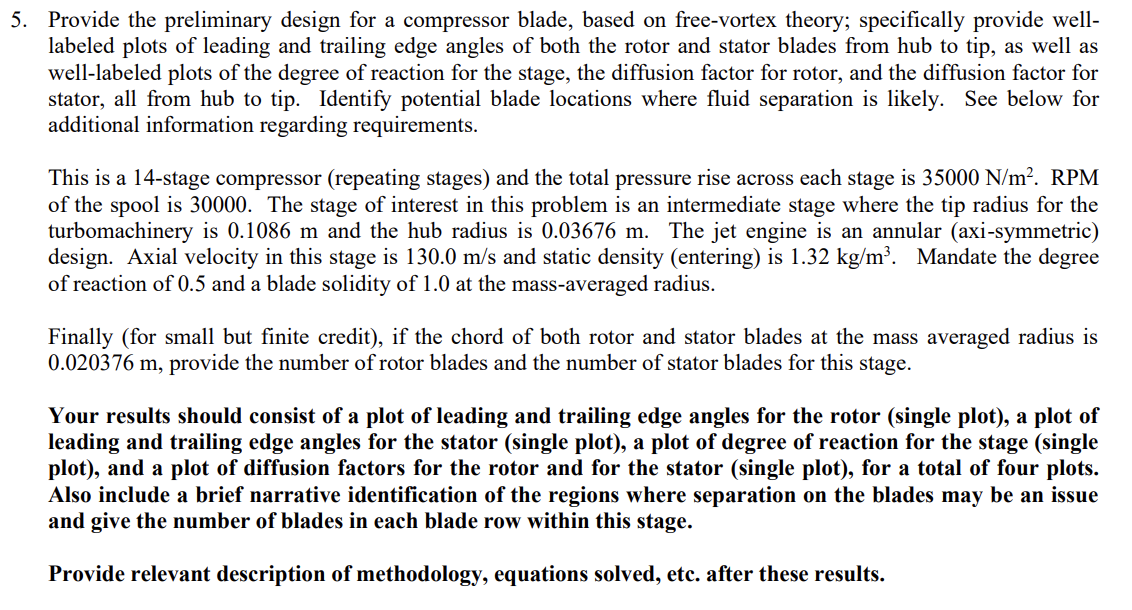
\includegraphics[width=1\textwidth]{images/5.png}
\end{figure}



\noindent Radius values spaced linearly between the hub and tip radius:
\begin{equation*}
    r = linspace(r_h, r_t, N_{steps})
\end{equation*}

\noindent Degree of reaction at a given location:
\begin{equation*}
    ^\circ R = 1 - \frac{r_m^2}{r^2} \left(1 - ^\circ R_m\right)
\end{equation*}

\noindent Where:

\begin{equation*}
    r_m = \sqrt{\frac{r_t^2 + r_h^2}{2}}
\end{equation*}

\noindent Degree of reaction at the hub:
\begin{equation*}
    ^\circ R_h = ^\circ R[0]
\end{equation*}

\noindent Swirl velocity equations:
\begin{equation*}
    V_{\theta_1 h} = \frac{w_0}{2} \left[\frac{2 \omega r_h}{w_0}\left(1 - ^\circ R_h\right) - \frac{1}{\frac{\omega r_h}{w_0}} \frac{\Delta P_t}{\rho_0 w_0^2} \right]
\end{equation*}
\begin{equation*}
    V_{\theta_2 h} = \frac{w_0}{2} \left[\frac{2 \omega r_h}{w_0}\left(1 - ^\circ R_h\right) + \frac{1}{\frac{\omega r_h}{w_0}} \frac{\Delta P_t}{\rho_0 w_0^2} \right]
\end{equation*}
\begin{equation*}
    V_{\theta_1} = \frac{r_h V_{\theta_1 h}}{r}
\end{equation*}
\begin{equation*}
    V_{\theta_2} = \frac{r_h V_{\theta_2 h}}{r}
\end{equation*}

\noindent Equations for stator leading and trailing edge angles
\begin{equation*}
    \theta_1 = \tan^{-1}{\frac{V_{\theta_1}}{w_0}}
\end{equation*}
\begin{equation*}
    \theta_2 = \tan^{-1}{\frac{V_{\theta_2}}{w_0}}
\end{equation*}

\noindent Equations for rotor leading and trailing edge angles
\begin{equation*}
    \beta_1 = \tan^{-1}\left({\frac{\omega r}{w_0} - \frac{V_{\theta_1}}{w_0}}\right)
\end{equation*}
\begin{equation*}
    \beta_2 = \tan^{-1}\left({\frac{\omega r}{w_0} - \frac{V_{\theta_2}}{w_0}}\right)
\end{equation*}

\noindent Equation for rotor diffusion:
\begin{equation*}
    D_{rotor} = 1 - \frac{\cos(\beta_1)}{\cos(\beta_2)} + \frac{|\tan\beta_1 - \tan\beta_2|}{2 \sigma \cos\beta_1}
\end{equation*}


\noindent Equation for stator diffusion:
\begin{equation*}
    D_{stator} = 1 - \frac{\cos(\theta_2)}{\cos(\theta_3)} + \frac{|\tan\theta_3 - \tan\theta_2|}{2 \sigma \sec\theta_2}
\end{equation*}

\noindent Where:


\begin{equation*}
    \sigma = \frac{r_m}{r} \sigma_m
\end{equation*}

\begin{figure}[hbt!]
    \centering
    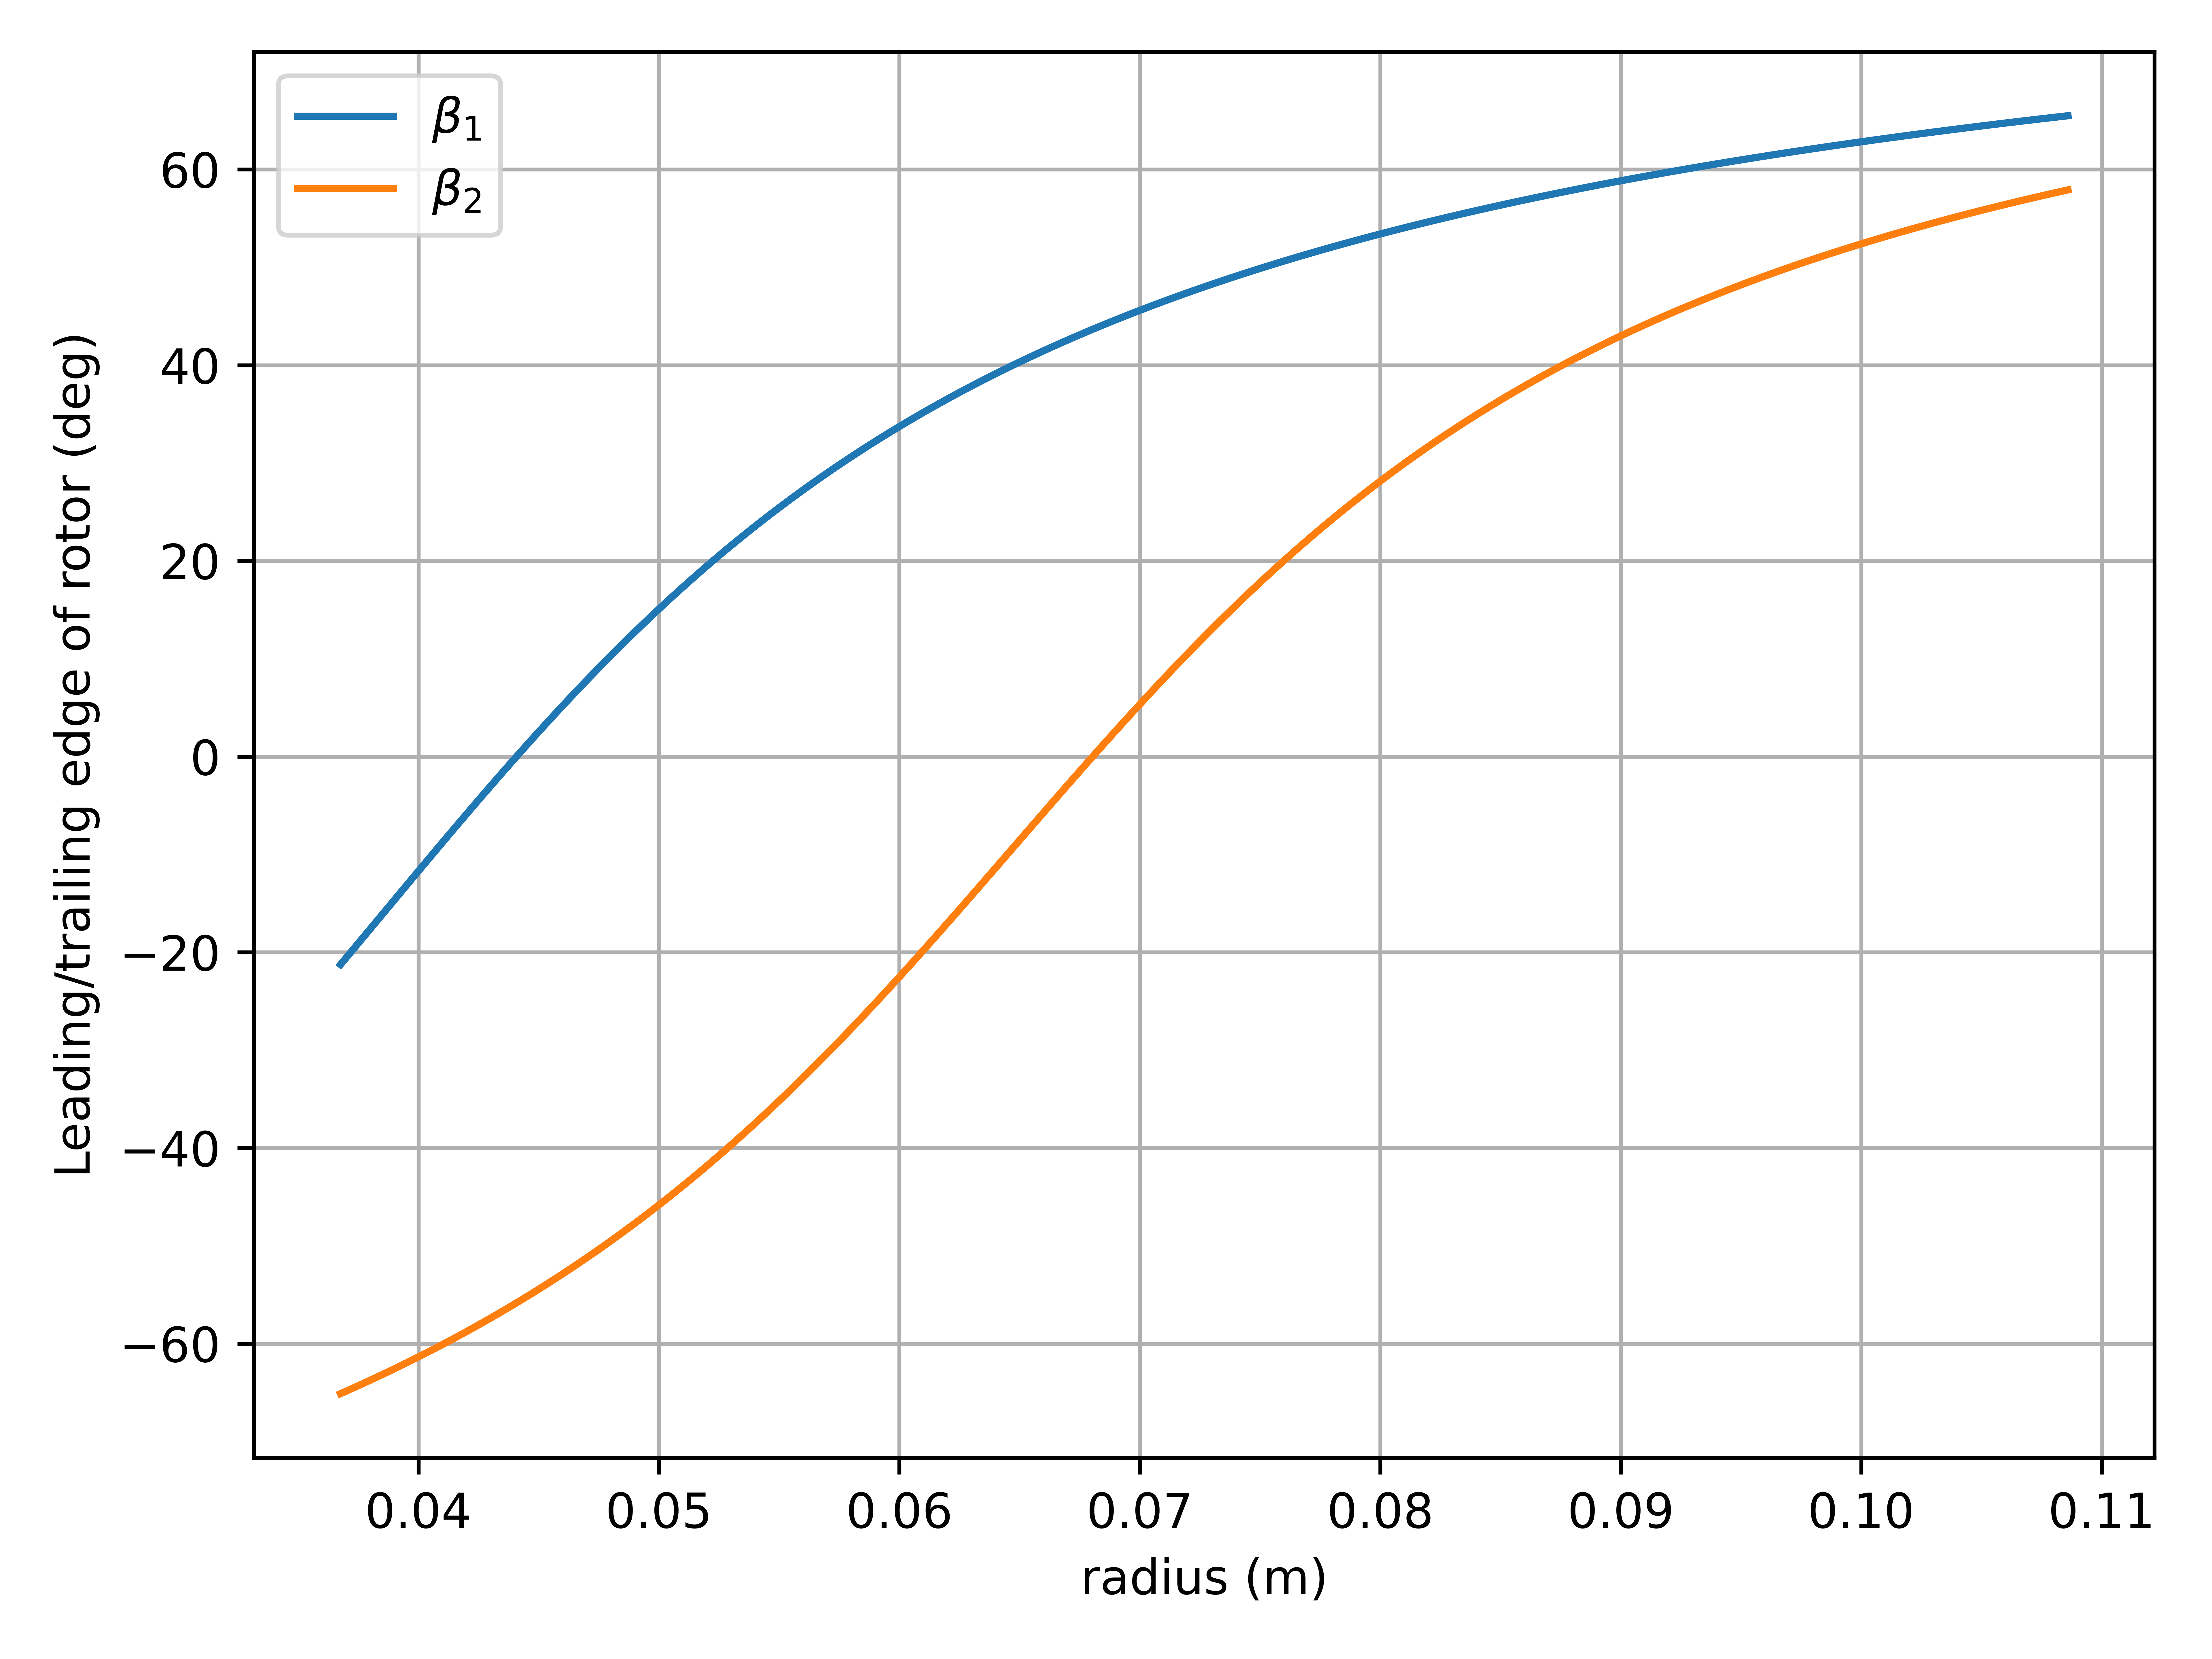
\includegraphics[width=.8\textwidth]{plots/rotor_angles.png}
\end{figure}

\clearpage
\begin{figure}[hbt!]
    \centering
    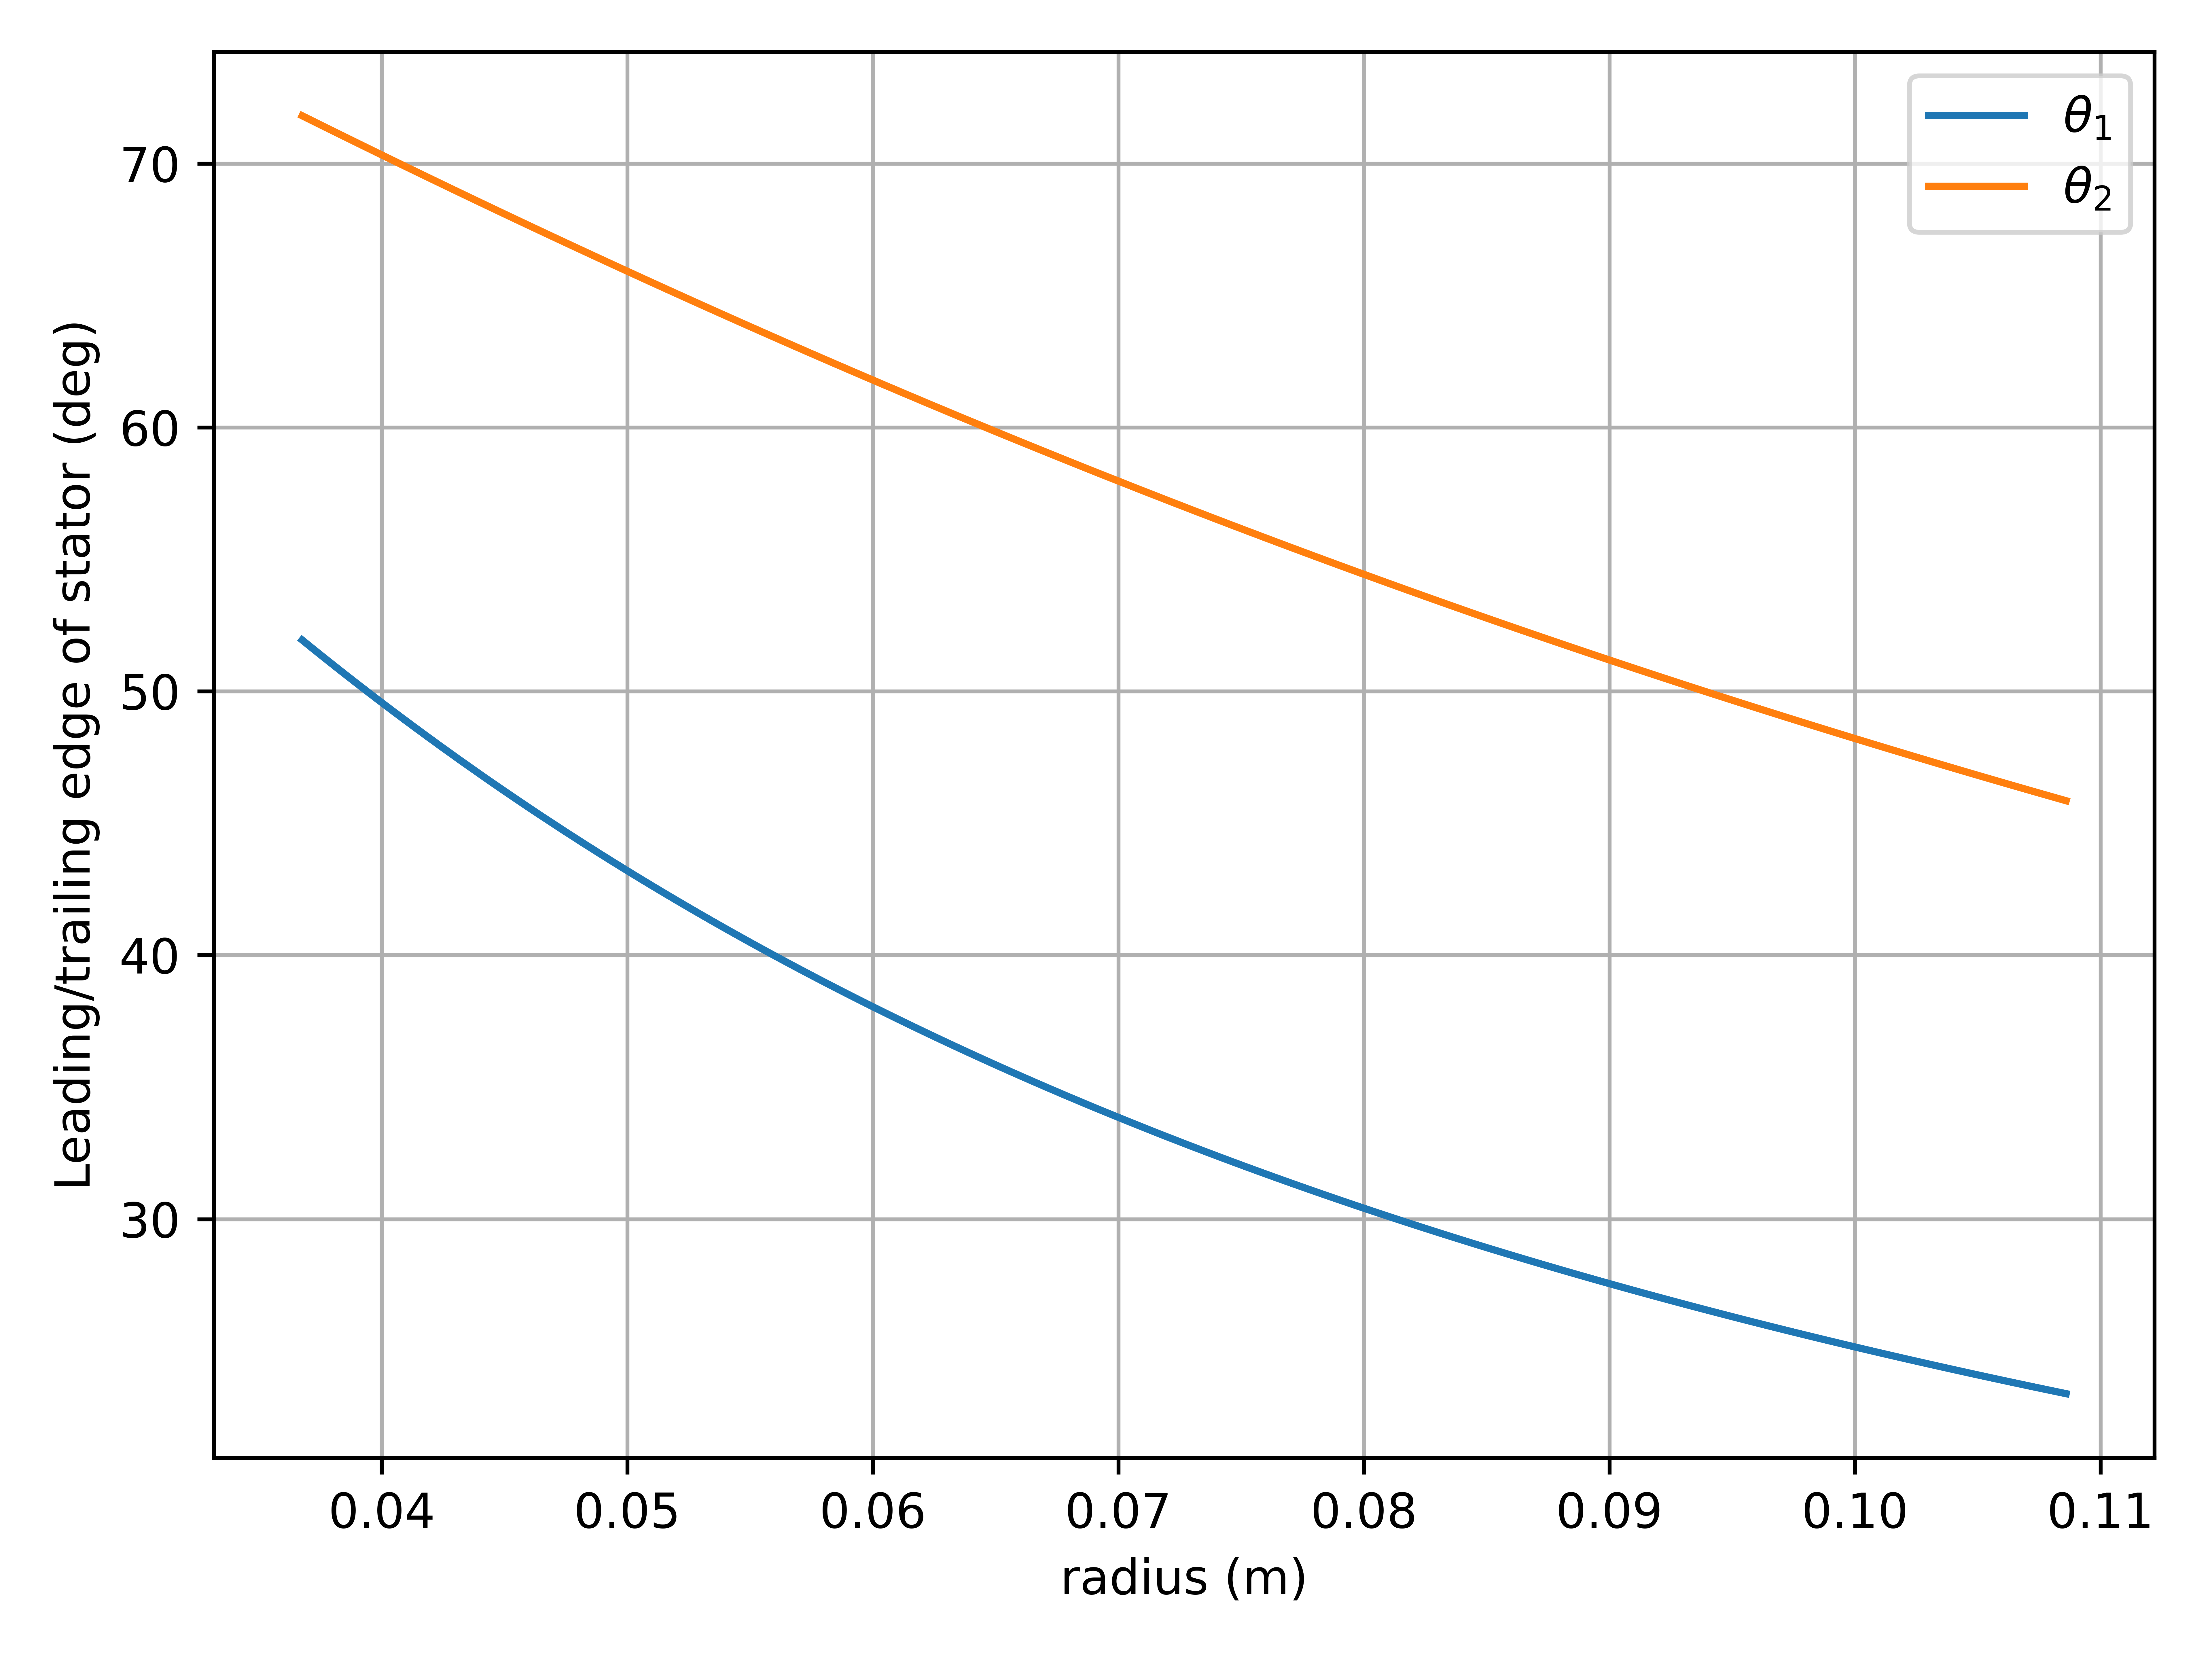
\includegraphics[width=.8\textwidth]{plots/stator_angles.png}
\end{figure}

\begin{figure}[hbt!]
    \centering
    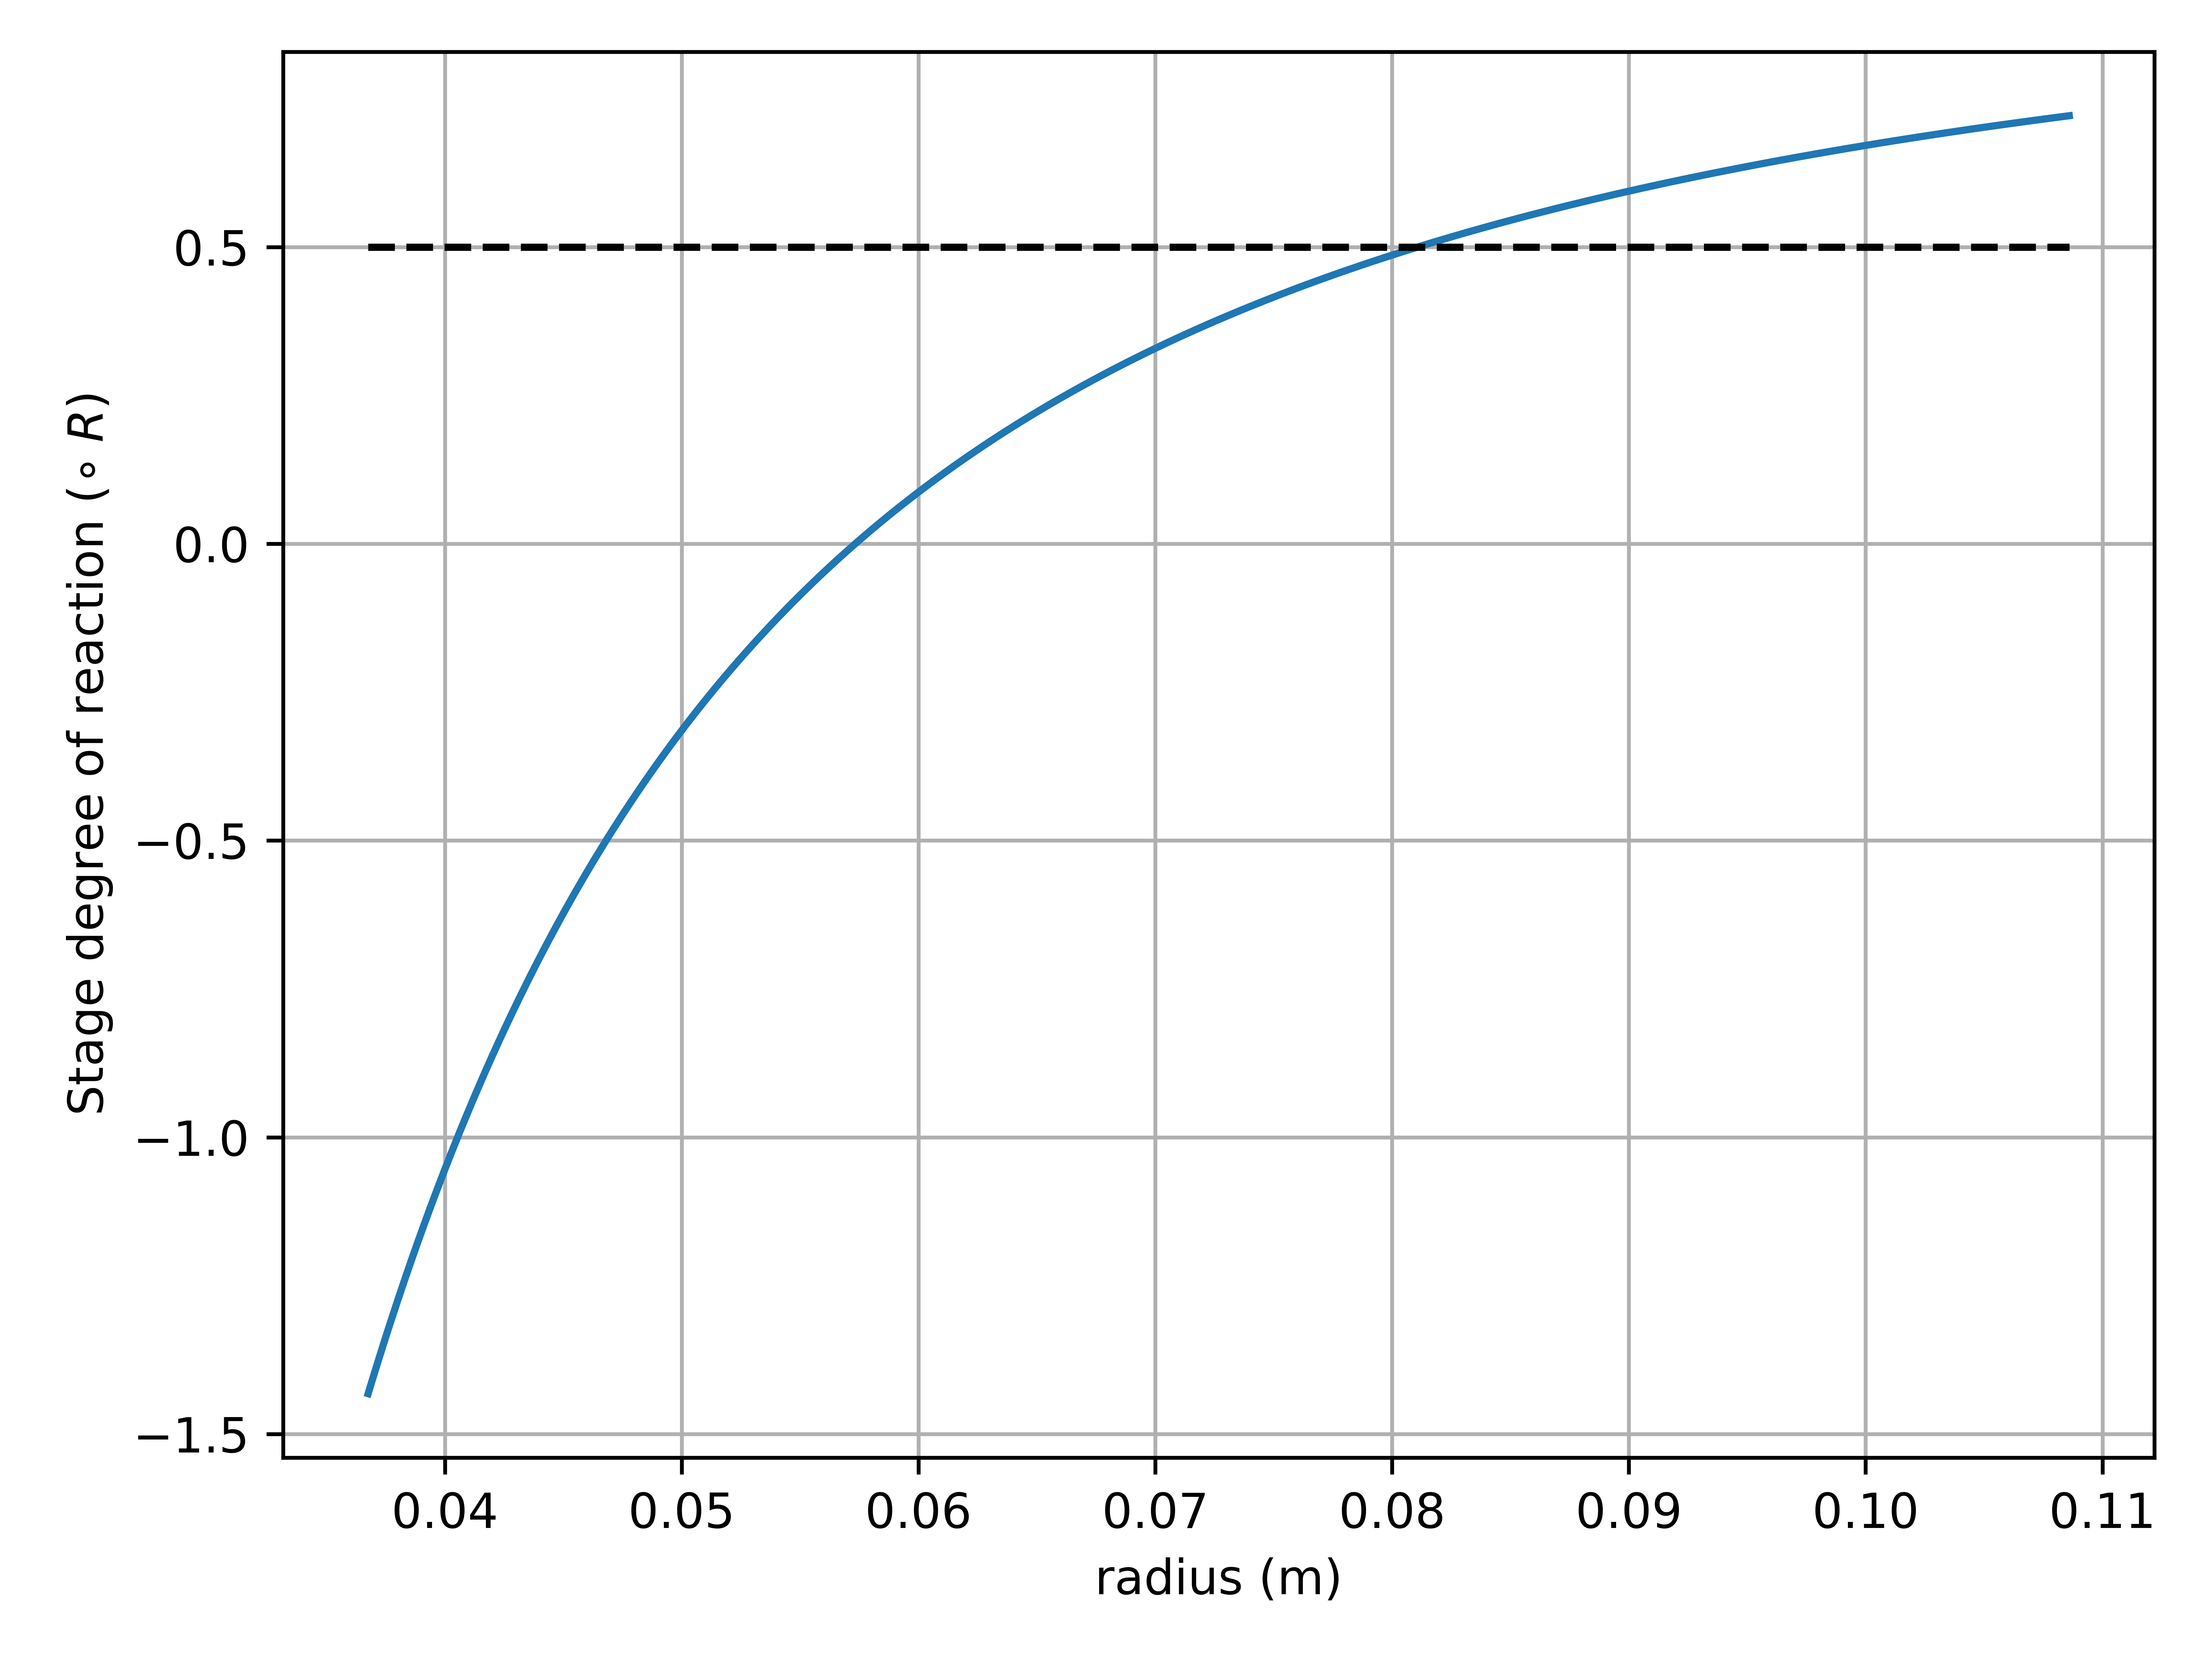
\includegraphics[width=.8\textwidth]{plots/dor.png}
\end{figure}

\clearpage
\begin{figure}[hbt!]
    \centering
    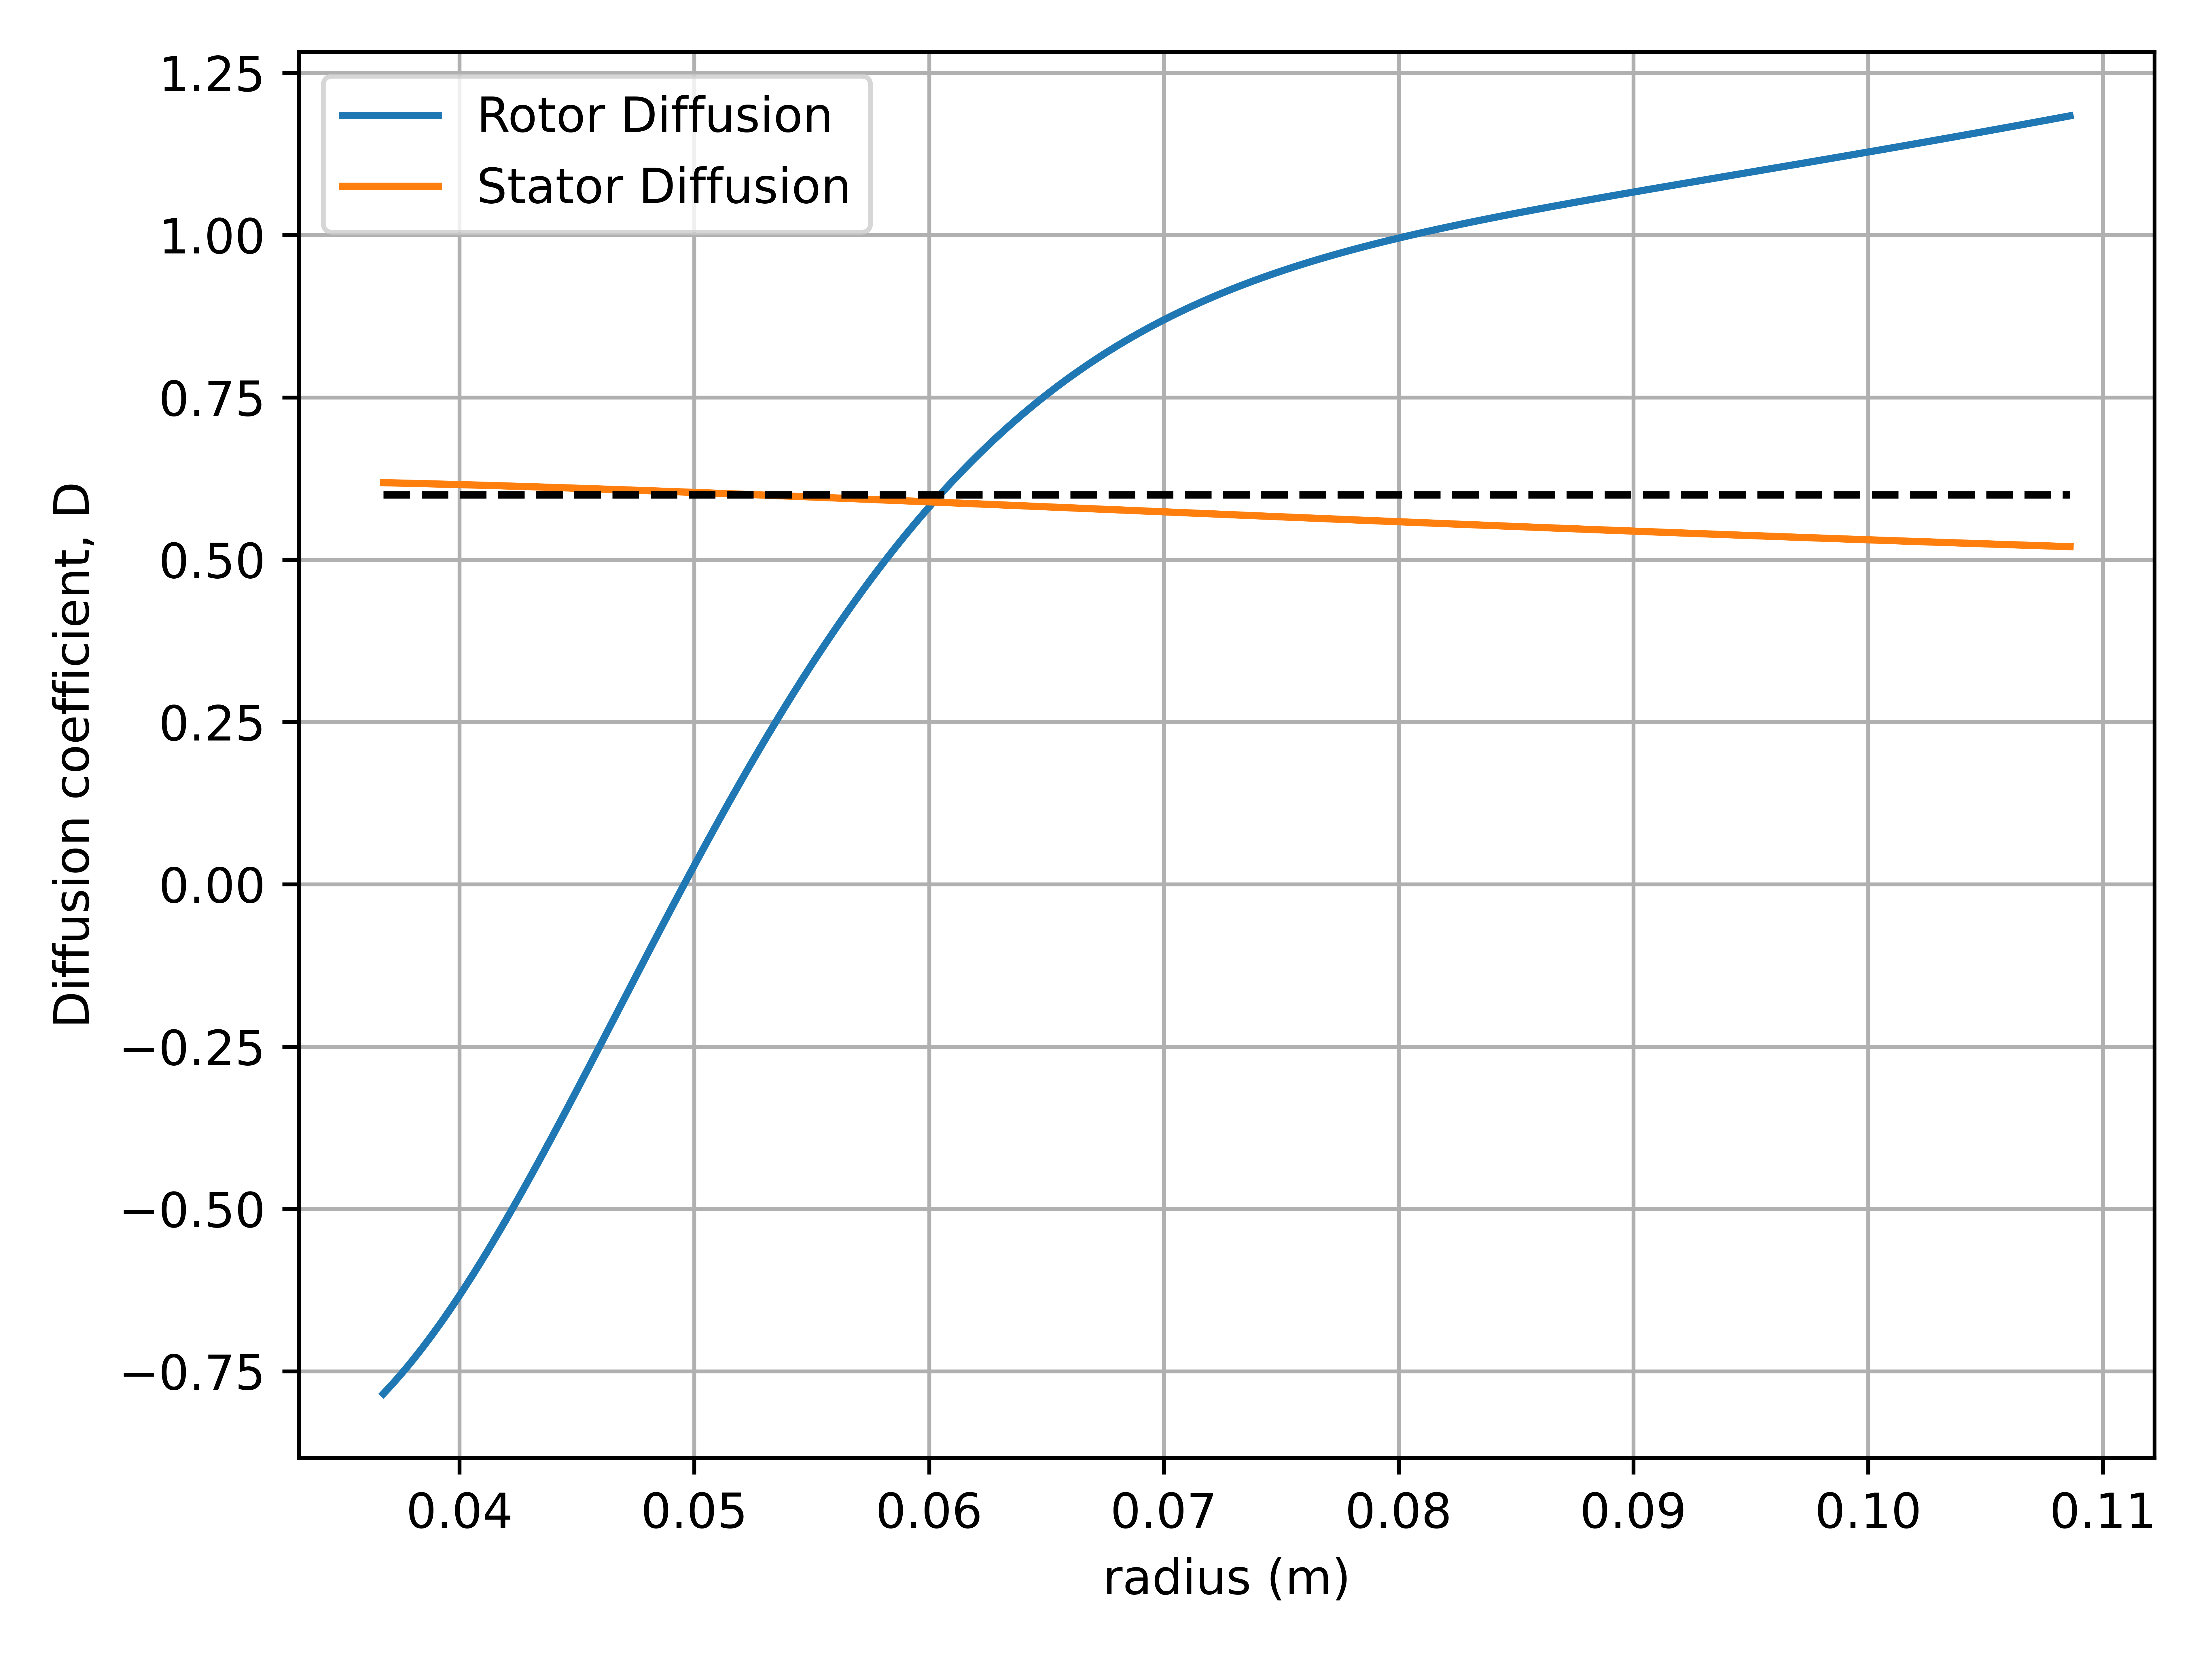
\includegraphics[width=.8\textwidth]{plots/diffusion.png}
\end{figure}

\noindent For the stator separation can occur at the hub and for the rotor separation will likely occur at $\boxed{r = 0.06}$ meters \\

\noindent There are 25 blades for the row in which the chord is given. This was solved by using the following equation:

\begin{equation*}
    blades = \frac{2 \pi r_m}{chord} = 25
\end{equation*}


\end{document}